\documentclass[12pt]{ctexart}
\usepackage{mathtools}
\begin{document}
    \title{王道计算机组成原理笔记}
    \author{王艺霖}
    \maketitle

\newpage

\section{检验码}
\subsection{循环冗余检验码(CRC码)}
\paragraph{CRC码的基本思想}~{}
\begin{enumerate}
    \item 数据发送、接收方约定一个“除数”
    \item K个信息位+R个检验位作为“被除数”,添加检验位后需保证除法的余数为0
    \item 收到数据后,进行除法检查余数是否为0,若余数非0说明出错,则进行重传或者纠错
\end{enumerate}


\paragraph{如何构造}~{}

模2除法介绍:
\begin{enumerate}
    \item 被除数首位为1时,商为1;被除数首位为0时,商为0;
    \item 每一步得到的余数都要抛弃首位;
    \item 若新的被除数首位(即已抛弃首位的余数)为0,除数为0。
\end{enumerate}


\paragraph{如何检查纠错}~{}

CRC是一种检错方法,而FCS是添加在数据后面的冗余码,在检错方法上可以选用CRC,但也可以不选用CRC。

在接受端把接收到的数据以帧为单位进行CRC检验:把收到的每一个帧都除以同样的除数P(模2运算),然后检查得到的余数R。


补码的真值0,只有一种表示形式
\paragraph{备注}~{}

K个信息位, R个检验位,若生成多项式选择得当,且$2^{R} >= K + R + 1$,可纠正1位错误。

原因为R位可以表示出$2^{R}$种状态,其中有$2^{R}-1$种错误的状态,而有$K+R$位

理论上可以证明循环冗余码的检错能力有以下特点:
\begin{enumerate}
    \item 可检测出所有奇数个错误
    \item 可检测出所有双比特的错误
    \item 可检测出所有小于等于检验位长度的连续错误
\end{enumerate}

\newpage
\section{定点数}

\subsection{定点数vs浮点数}
定点数小数: 位数固定  \hspace{15ex}3.14

浮点数小数:位数不固定 \hspace{13ex}$3.14 * 10^{2}$

\paragraph{无符号数}~{}

整个机器字长的全部二进制位均为数值位,没有符号位,相当于数的绝对值


表示范围:


8位二进制数:$2^{8}$种不同的状态

$
\quad 00000000~1111 1111 = 100000000-1
$


n位的无符号整数表示范围为:0到$2^{n}-1$

\paragraph{有符号数的定点表示}~{}

定点整数:\hspace{3ex} 符号位,数值部分,小数点位置

定点小数:\hspace{3ex} 符号位,小数点位置,数值部分

\paragraph{原码}~{}

原码:用尾数表示真值的绝对值,符号位“0/1”对应“正/负”

若机器字长为$n+1$位,那么表示的数的范围为:$-2^{n}+1 ~ 2^{n}-1$
\paragraph{反码}~{}

若符号位为0, 则反码与原码相同

若符号位为1, 则\textbf{数值位}全部取反

真值有\textbf{+0}和\textbf{-0}两种

\paragraph{补码}~{}
\begin{enumerate}
    \item 正数的补码=原码
    \item 负数的补码=反码末尾+1
    \item 0的补码只有一种真值形式00000000
    \item 定点整数:[X]补 = 1,0000000 表示X=$2^7$
    \item 若机器字长$n+1$位,补码整数的表示范围:$-2^n<=x<=2^n-1$
    \item 定点小数补码[X]补 =1.0000000 表示X=-1
    \item 若机器字长为n+1位,补码小数的表示范围:$-1<=x<=1-2^{-n}$(比原码多一个-1)
\end{enumerate}

\paragraph{移码}~{}

移码:补码的基础上将符号位取反。\textbf{注意:移码只能用于表示整数}

\subsection{各种码的作用}~{}

\paragraph{模运算的性质}~{}

带余除法——$x,m \in Z, m > 0$则存在唯一决定的整数q和r使得:

$x = q*m + r$

加法或者减法运算:

$a+b$为a+b的补码

\paragraph{移位运算}~{}

\textbf{原码}的算术移位——符号位保持不变,仅对数值为进行移位

右移:高位补0,低位舍弃。若舍弃的位=0,则相当于/2若舍弃的位不等于0,则会舍弃精度。

左移:地位补0,高位舍弃。若舍弃的位=0,则相当于*2,否则会出现严重误差。

\textbf{反码}的算术移位——正数的反码与原码相同,因此对正数反码的移位运算也和原码相同。

右移:高位补0,低位舍弃

左移:低位补0,高位舍弃

\textbf{负数}的移位:

右移:高位补1,地位舍弃

左移:低位补1,高位舍弃

\textbf{补码}的算术移位:

\textbf{补码}的算术移位——正数的补码与原码相同:因此对正数反码的移位运算也和原码相同

右移:高位补0,低位舍弃
左移:低位补0,高位舍弃

\textbf{负数}补码=反码末尾+1导致反码最右边几个连续的1都因为进位而变为0,直到进位碰到第一个0为止


规律:——负数补码中,最右边的1及其右边同原码。最右边的1的左边同反码


\textbf{算术移位的应用举例}:快速幂

\textbf{逻辑移位}:

逻辑右移:高位补0,低位舍弃
逻辑左移:低位补0,高位舍弃

\textbf{逻辑移位的应用举例}:RGB

\textbf{循环移位}:
CF位来存储进位:在左移或者右移时补上。

\textbf{循环移位的应用举例}:高低字节的转换

\subsection{加减运算和溢出判断}
加法器直接对原码进行加法运算,可能出错

在这里阐述一下基本的原理是什么,首先对于一个负数取补码相当于把它变为了自己的补数

假设我们求解 15 - 10 ,此时15还是15,而-10则会变为$256-10=246$,原来的往后移动10位,
等价于15 + 246以后移动的位置,思想和钟表差不多,这个时候我们变回原码就可以了。

对于补码来说,无论加法还是减法,最后都会转变位加法,由加法器实现运算,
符号位也参与运算。

\textbf{溢出判断}
\begin{figure}[htbp]
    \centering
    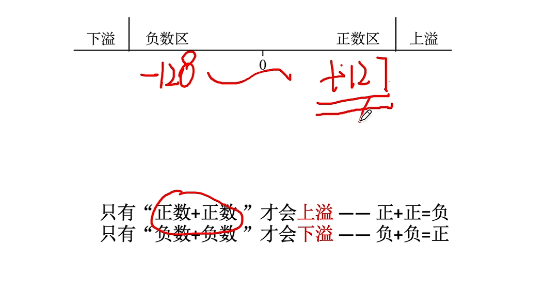
\includegraphics[scale=0.6]{溢出判断.png}
    \caption{溢出判断}
    \end{figure} 

具体判断后面再去看

\subsection{原码的乘法运算}

手动乘法的本质在于r进制,具体内容不再赘述。

同理得到手动二进制乘法

设机器字长位n+1=5位,含有1位符号位,$[x]$的原码为1.1101,
$y$的原码为0.1011,采用原码一位乘法求$x*y$。

\textbf{原码乘法}
\begin{figure}[htbp]
    \centering
    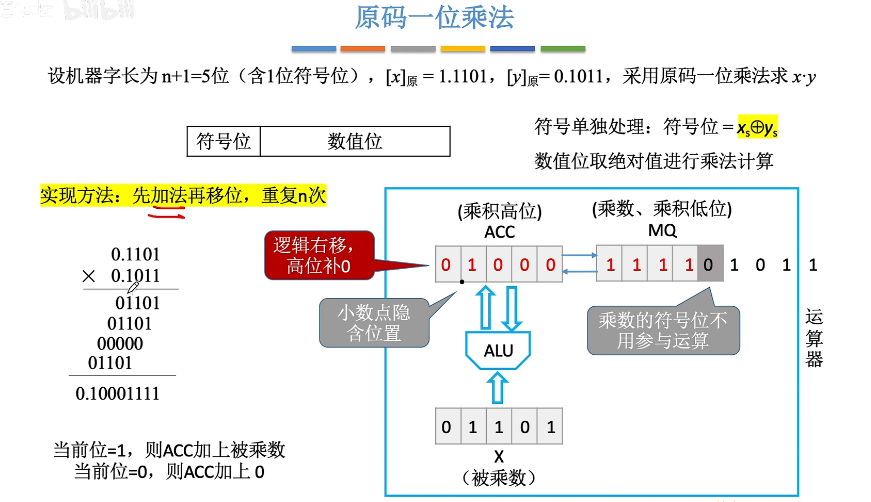
\includegraphics[scale=0.6]{原码乘法.png}
    \caption{原码乘法}
    \end{figure} 

\subsection{补码的一位乘法运算}
设机器字长为5位(含有1位符号位,n=4),x = -0.1101, y = +0.1011,
采用Boooth算法求x*y,
x的补码为1.0011,-x的补码为0.1101,y的补码为0.1011

补码的一位乘法:
进行n轮加法,移位,最后再多来一次加法。

符号位参与运算 

辅助位 - MQ中最低位=1时,(ACC)+ x的补码

辅助位 - MQ中最低位=0时,(ACC)+0

辅助位 - MQ中最低位=-1时,(ACC)+ -x的补码

\textbf{补码乘法}
\begin{figure}[htbp]
    \centering
    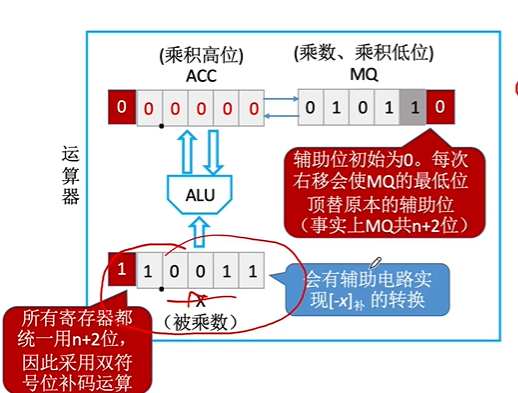
\includegraphics[scale=0.6]{补码乘法.png}
    \caption{补码乘法}
    \end{figure} 
\textbf{手工模拟计算}
    \begin{figure}[htbp]
        \centering
        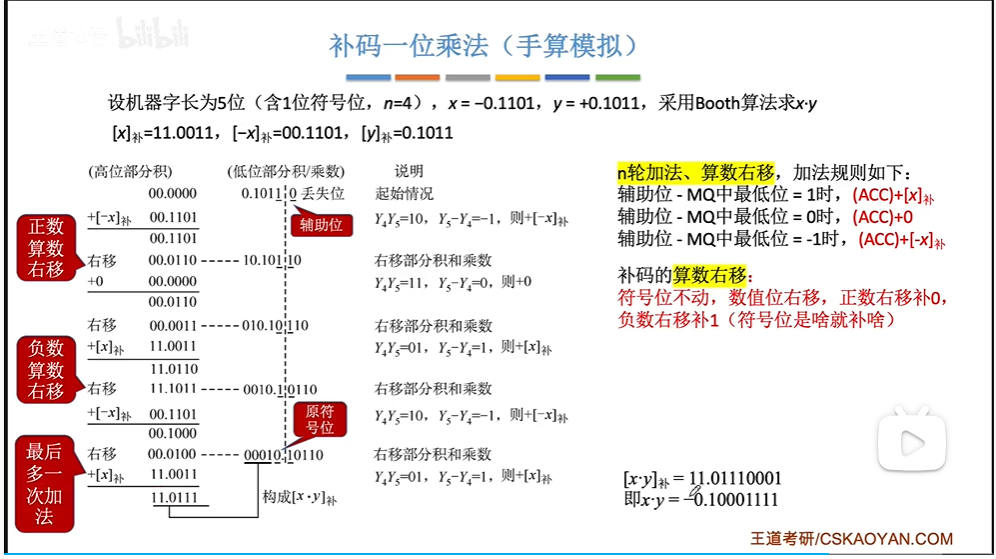
\includegraphics[scale=0.6]{模拟计算.png}
        \caption{模拟计算乘法}
        \end{figure} 

\subsection{原码的除法如上图}
\begin{figure}[htbp]
    \centering
    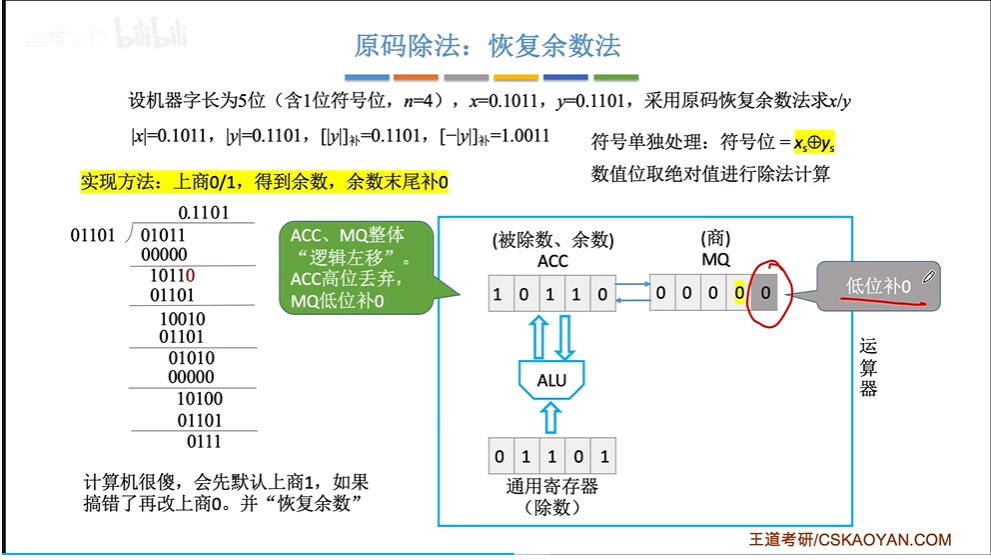
\includegraphics[scale=0.6]{原码除法.png}
    \caption{原码除法}
    \end{figure} 

\begin{figure}[htbp]
        \centering
        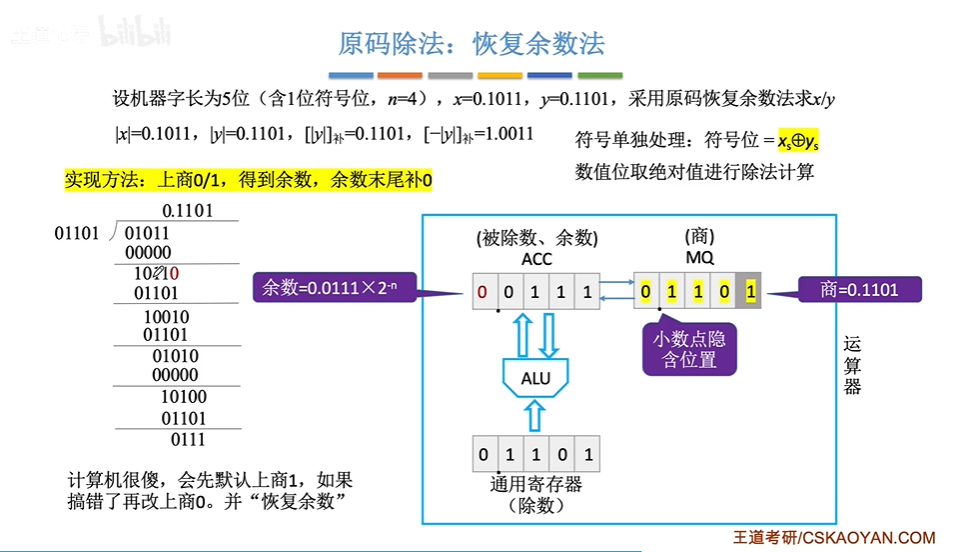
\includegraphics[scale=0.6]{原码除法1.png}
        \caption{原码除法1}
        \end{figure} 
\begin{figure}[htbp]
        \centering
        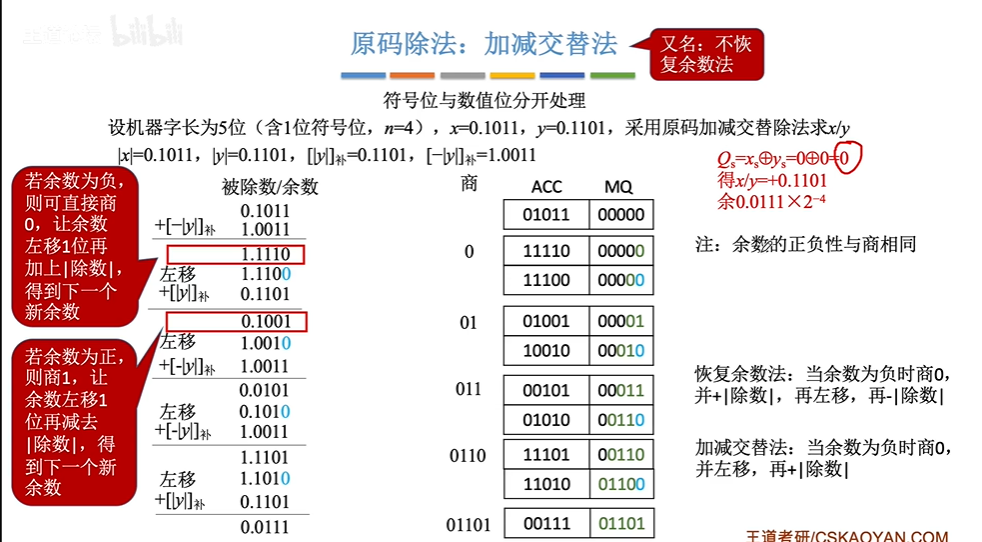
\includegraphics[scale=0.6]{加减交替法.png}
        \caption{加减交替法}
        \end{figure} 
\subsection{数据存储与排列}
多字节数据在内存里面一定是占连续的几个字节。

分为大端方式和小端方式:

大端方式--便于人类阅读 从高到低

小端方式--便于机器处理 从低到高

\textbf{边界对齐}
现代计算机通常是按字节编址,即每个字节对应1个地址。
通常也支持安字,按半字,按字节寻址。

假设存储字长为32位,则一个字=32bit,半字=16bit。
每次访存只能读/写1个字。

现代计算机分为边界对齐和边界不对齐的方式。

边界对齐只需要一次访存(空间换时间)

边界不对齐效率相对较低。

\subsection{浮点数的表示和运算}
定点数的局限性:

比如我的财富位-8540,可以用2B定点整数short即可表示。

马云的财富:10000000000000

4B定点整数int$....$都表示不了

定点数可表示的数字范围有限,但是我们不能无限制地增加数据。

从科学计数法理解浮点数:

普通计数法: $302657264536$

科学计数法:

$+3.026 * 10 ^{11}$
可以表示为 $+11 +3.026$

浮点数的真值: $ N = r ^  E * M$

阶码:常用补码或者移码表示的定点整数

尾数:常用原码或者补码表示的定点小数

例:阶码,尾数均用补码表示,求a,b的真值
$a = 0,-1;1.1001$
$b = 0,10;0.001001$
a: 阶码0,01对应真值+1, 尾数1.1001对应真值-0.0111 = $-(2^{-2}+2^{-3}+2^{-4})$
a的真值=$2^1 * (-0.0111)$ = -0.111 

规格化浮点数:规定尾数的最高位数值位必须是一个有效值

左规: 当浮点数运算的结果位非规格化时要进行规格化处理。
将尾数算数左移1位,阶码减1

右规: 当浮点数运算的结果尾数出现溢出(双符号位为01或者10)时,将尾数算术右移一位,
阶码+1

规格化浮点数的特点:
1. 用原码表示的尾数进行规格化
正数用$0.1 * ***$的形式,其最大值的表示为$0.111111$,最小值
表示为$0.10...0$。
尾数的表示范围为$1/2<=M<=(1-2^{-n})$.

负数的表示范围为$1.1*****$的形式,其最大值表示为$1.100...0$,最小值
尾数的表示范围为$-(1-2^{-n})<=M<=-1/2$。

用\textbf{补码}的不再赘述。
\begin{figure}[htbp]
    \centering
    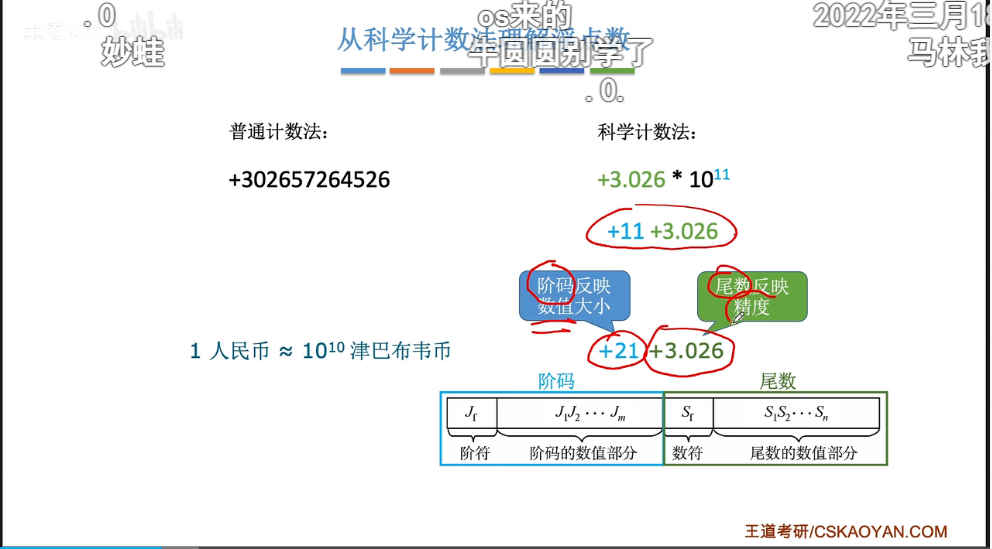
\includegraphics[scale=0.6]{从科学计数法理解浮点数.png}
    \caption{从科学计数法理解浮点数}
    \end{figure}
\subsection{$IEEE 754$}
移码:补码的基础上将符号位取反。
移码只能表示整数

移码的定义:移码=真值+偏置值
\begin{figure}[htbp]
    \centering
    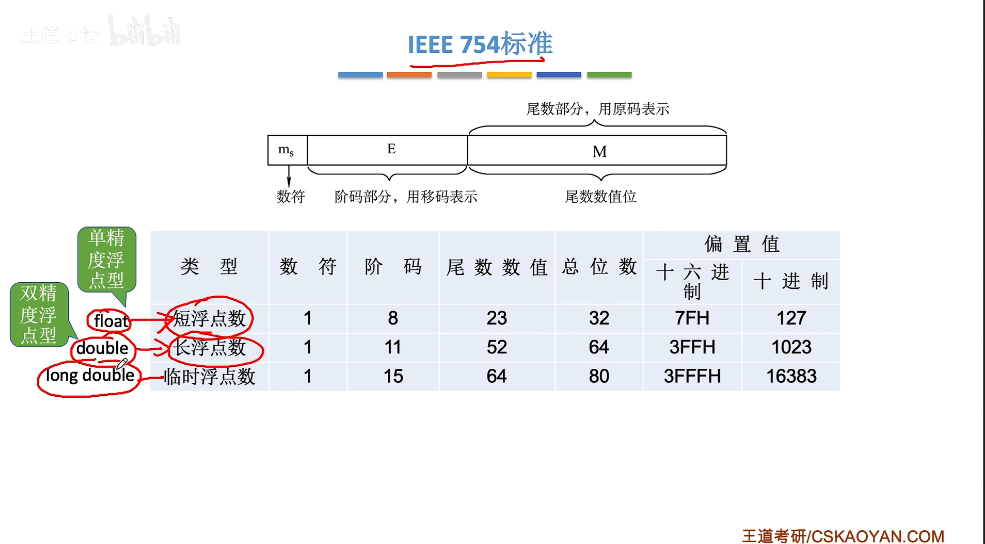
\includegraphics[scale=0.6]{IEEE.png}
    \caption{IEEE标准}
    \end{figure}
这一部分也是简单了解

\subsection{浮点数的加减运算}
\begin{enumerate}
    \item 对阶 小阶向大阶靠齐(方便计算机对尾数处理)
    \item 尾数加减
    \item 规格化 即左规或者右规
    \item 舍入 若规定只能保留6位有效数,则多余的直接砍掉(四舍五入)
    \item 判溢出, 若规定阶码不能超过两位,若运算后超出范围,则溢出
\end{enumerate}
\subsection{电路的基本原理}
算术逻辑单元(ALU)
\begin{figure}[htbp]
    \centering
    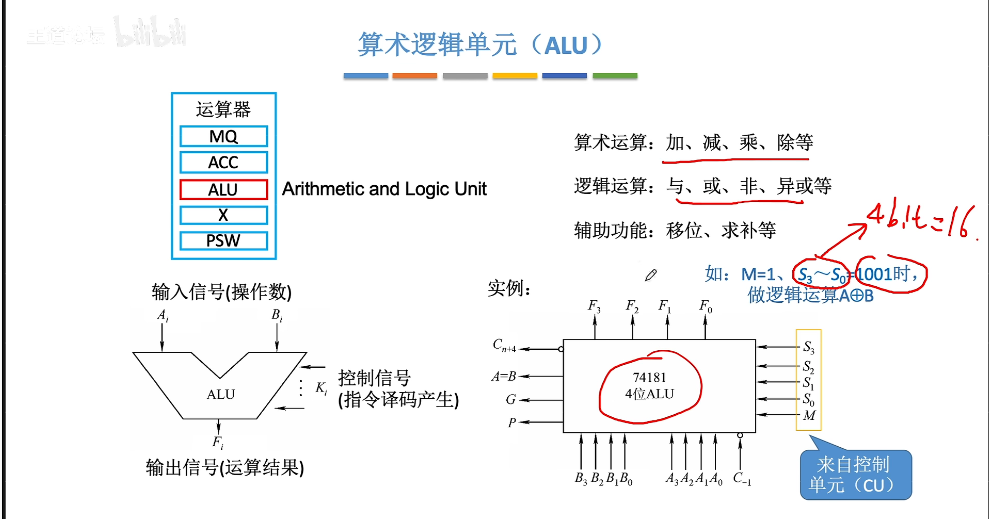
\includegraphics[scale=0.6]{算术逻辑单元.png}
    \caption{算术逻辑单元(ALU)}
    \end{figure}
基本逻辑(门电路)暂时不看

回忆:奇偶校验码

逻辑表达式是对电路的数学化描述。

一位全加器

本位和等概念,这里使用异或运算实现的。

串行加法器:只有一个全加器,数据逐位串行送入加法器进行运算。
进位触发器用来寄存进位信号,以便参与下一次运算。

串行进位的并行加法器:把n个全加器串接起来,就可以进行两个n位数的相加。
每一级进位直接依赖于上一级的进位,即进位信号是逐级形成的。

\subsection{加法器和ALU的改进}
不用太认真看

\subsection{分类及发展方向}
电子计算机分为电子模拟计算机和电子数字计算机。

电子数字计算机分为专用计算机和通用计算机。通用计算机又分为大型机,小型机,
单片机等。

指令和数据流:
\begin{enumerate}
    \item 单指令流和单数据流:冯诺依曼体系结构
    \item 单指令流和多数据流:陈列处理器,向量处理器
    \item 多指令流和单数据流:实际上不存在
    \item 多指令流和多数据流:多处理器,多计算机
\end{enumerate}

\subsection{计算机系统的组成}
这是计算机系统的组成
\begin{figure}[htbp]
    \centering
    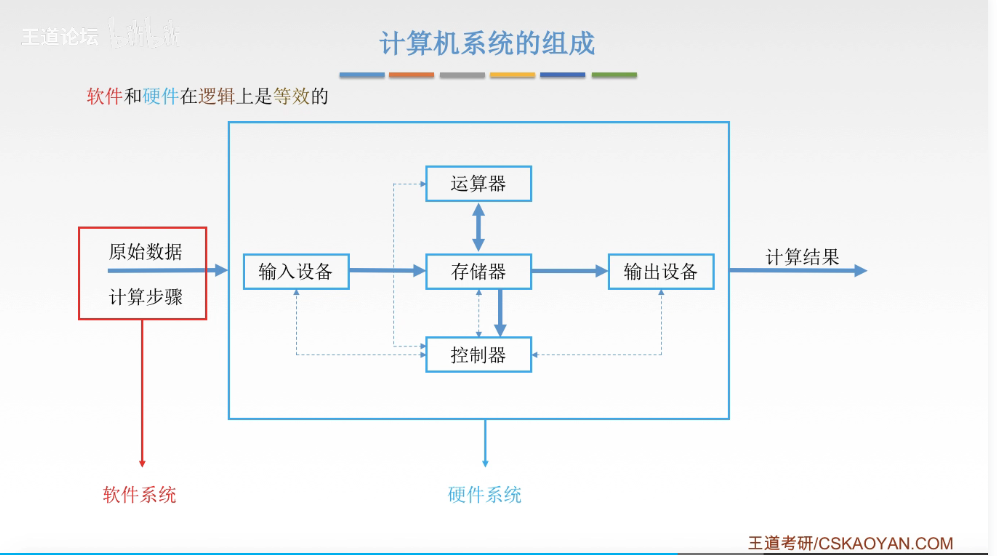
\includegraphics[scale=0.6]{计算机系统的组成.png}
    \caption{计算机系统的组成}
    \end{figure}
主机包括运算器和控制器(CPU)和主存储器,这个和传统意义的主机是区别的。

输入设备和输出设备称为I/O设备

辅助存储器

\subsection{功能部件-I/O设备}
外设包括:输入设备,输出设备以及辅助存储器

\subsection{软件系统}
软件分为系统软件和应用软件

系统软件:整理整个计算机系统,使得系统资源得到合理调度:
操作系统(OS),数据库管理系统(DBMS),语言处理系统

应用软件,完成用户的特定任务,使用系统软件提供的资源接口。
\begin{enumerate}
    \item 机器语言:二进制代码  
    \item 汇编语言
    \item 高级语言:C/C++、java,整段编译和解释程序两种
\end{enumerate}

\subsection{计算机系统的层次结构}
虚拟机器M4(高级语言机器)-----虚拟机器M3(汇编语言机器)----虚拟机器M2(操作系统机器)
-----传统机器M1(用机器语言的机器)
----微程序机器M0(微指令系统)

\subsection{存储器}

主存储器位于主机中,和运算器与控制器一起。

辅助存储器又被称为外存。
\begin{figure}[htbp]
    \centering
    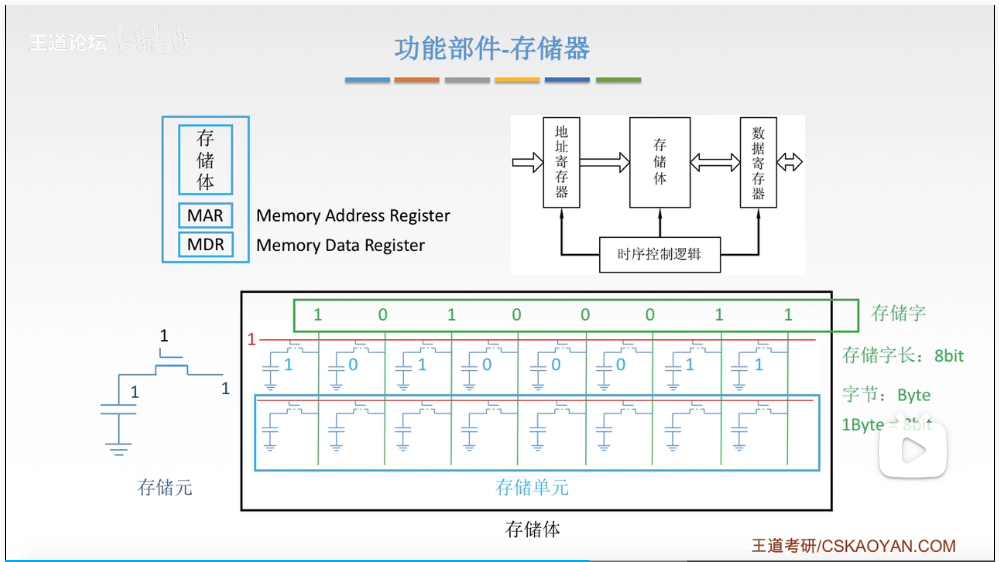
\includegraphics[scale=0.6]{存储器.png}
    \caption{功能部件-存储器}
    \end{figure}

\begin{figure}[htbp]
        \centering
        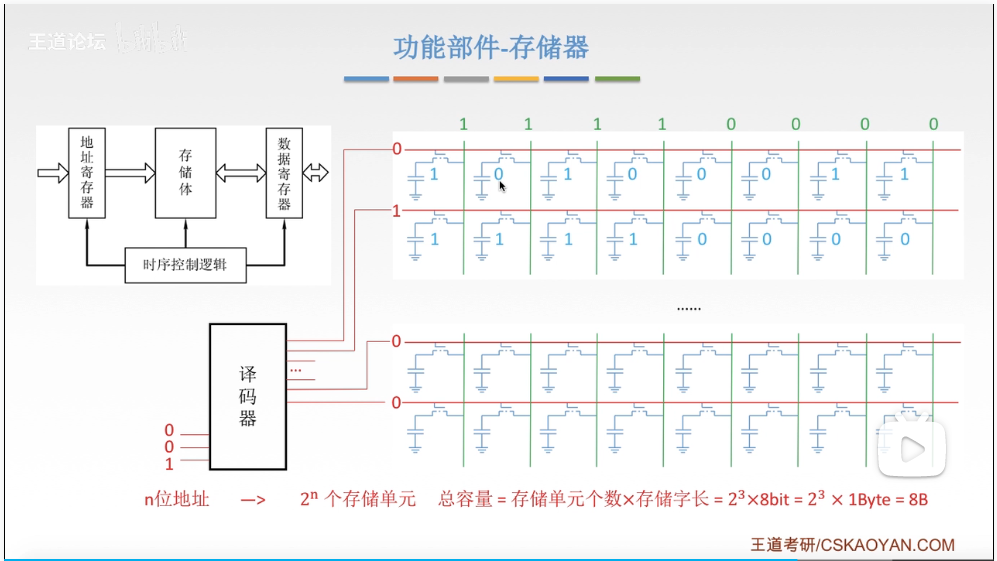
\includegraphics[scale=0.6]{存储器1.png}
        \caption{功能部件-存储器1}
        \end{figure}
\begin{figure}[htbp]
        \centering
        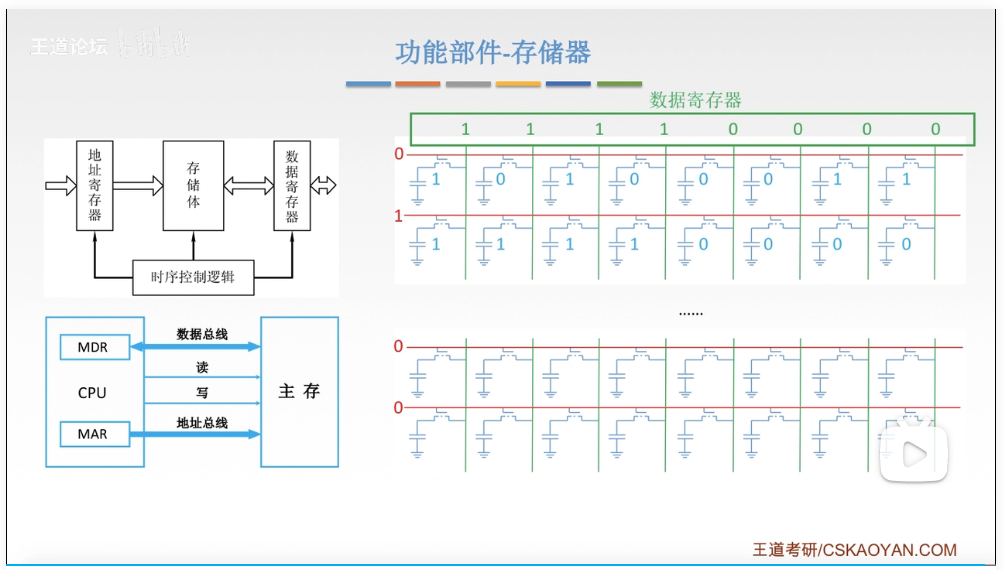
\includegraphics[scale=0.6]{存储器2.png}
        \caption{功能部件-存储器2}
        \end{figure}

\begin{figure}[htbp]
    \centering
    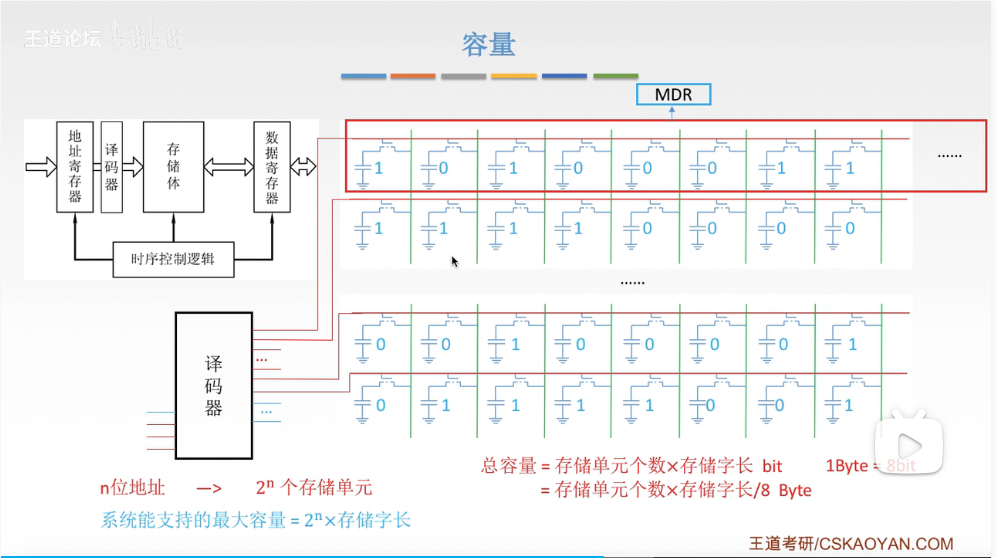
\includegraphics[scale=0.6]{容量.png}
    \caption{容量}
    \end{figure}
\subsection{半导体存储器RAM}

\begin{figure}[htbp]
    \centering
    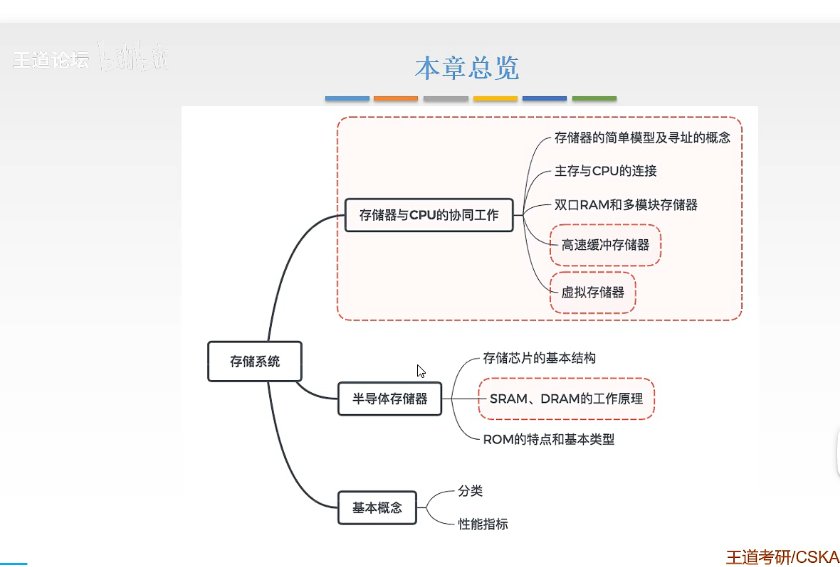
\includegraphics[scale=0.6]{存储.png}
    \caption{存储}
    \end{figure}
\begin{figure}[htbp]
    \centering
    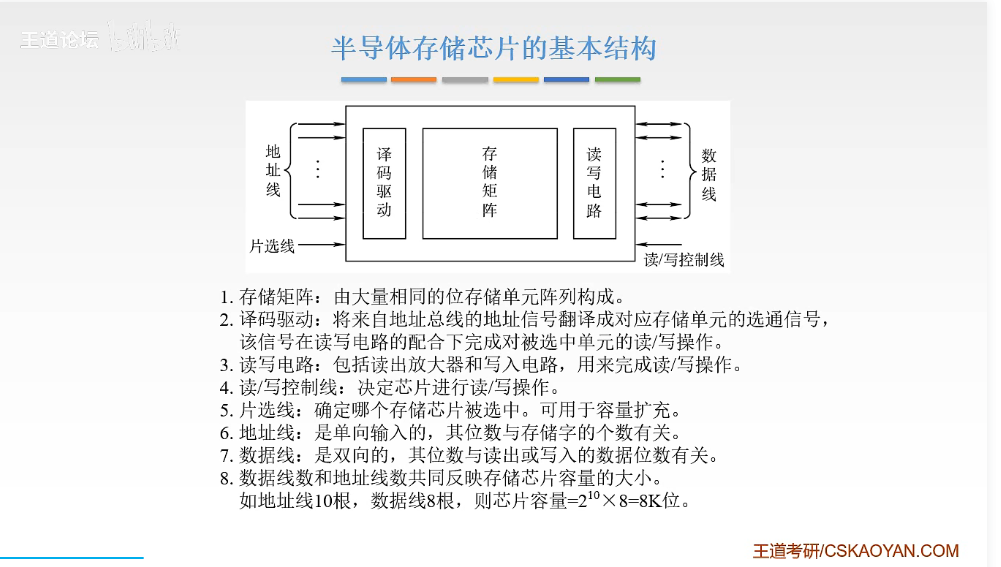
\includegraphics[scale=0.6]{基本结构.png}
    \caption{基本结构}
    \end{figure}
\begin{figure}[htbp]
    \centering
    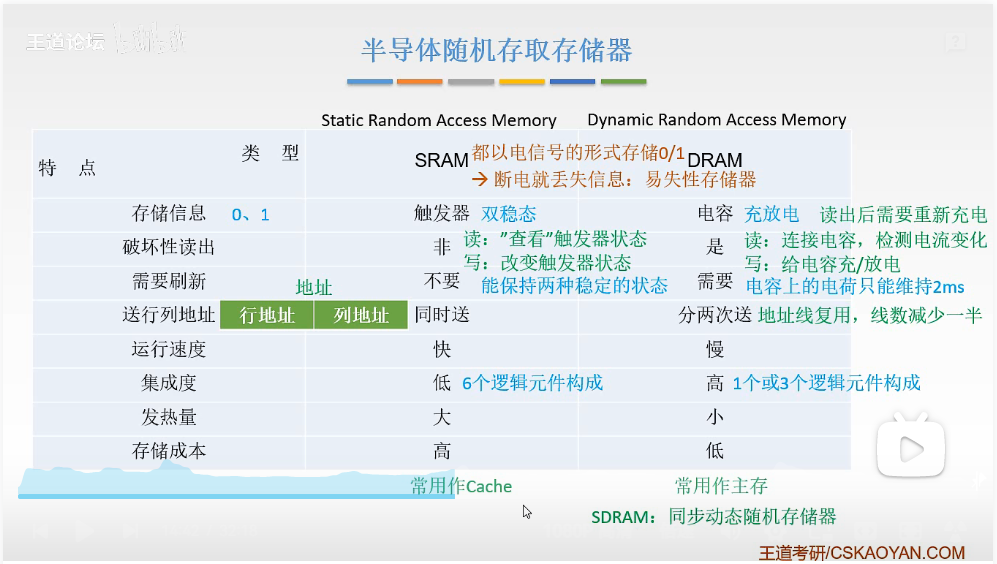
\includegraphics[scale=0.6]{半导体随机读取存储器.png}
    \caption{半导体随机读取存储器}
    \end{figure}
关于DRAM的刷新:
\begin{enumerate}
    \item 多久刷新一次:刷新周期为2ms
    \item 每次刷新多少存储单元?以行为单位,每次刷新一行存储单元
\end{enumerate}
\begin{figure}[htbp]
    \centering
    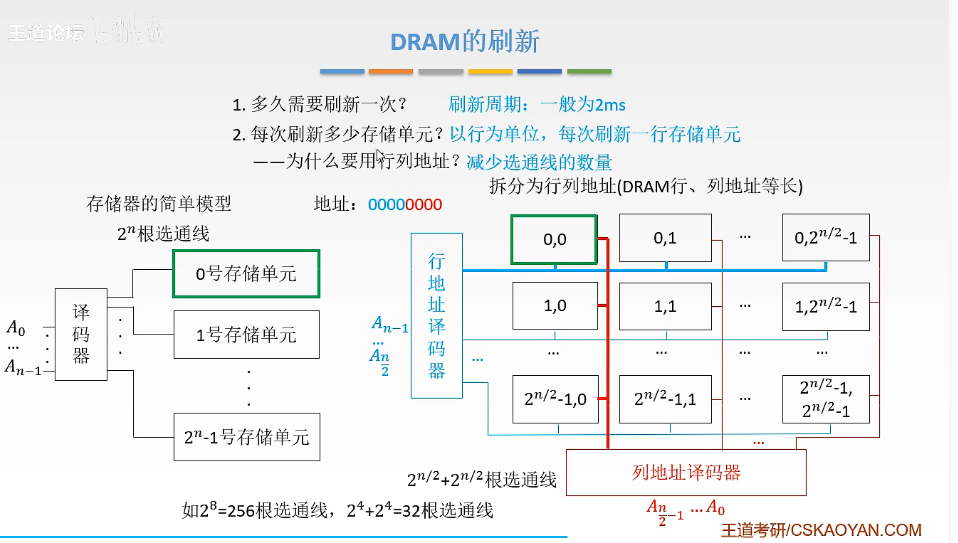
\includegraphics[scale=0.6]{DRM的刷新.png}
    \caption{DRM的刷新}
    \end{figure}
\begin{figure}[htbp]
    \centering
    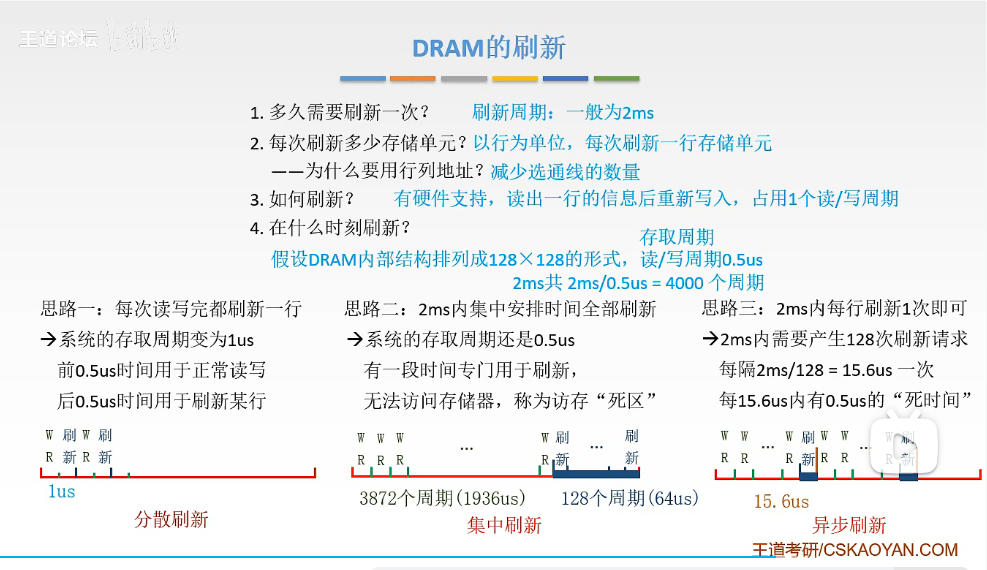
\includegraphics[scale=0.6]{DRM的刷新1.png}
    \caption{DRM的刷新}
     \end{figure}
\subsection{RAM-易失性存储器}
CPU的任务是到主存中取指令,按指令的指示进行下一步工作。
主存由RAM和ROM共同组成。
\begin{figure}[htbp]
    \centering
    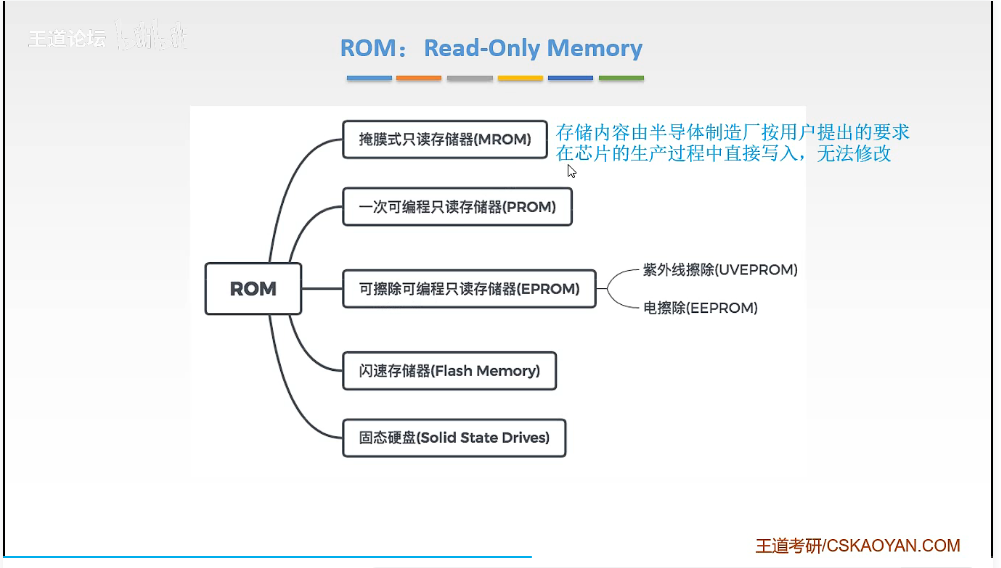
\includegraphics[scale=0.6]{ROM.png}
    \caption{ROM}
     \end{figure}
\subsection{主存与CPU的连接}
存取周期:启动存取,存取完,下次存取。(中间有恢复时间)
\begin{figure}[htbp]
    \centering
    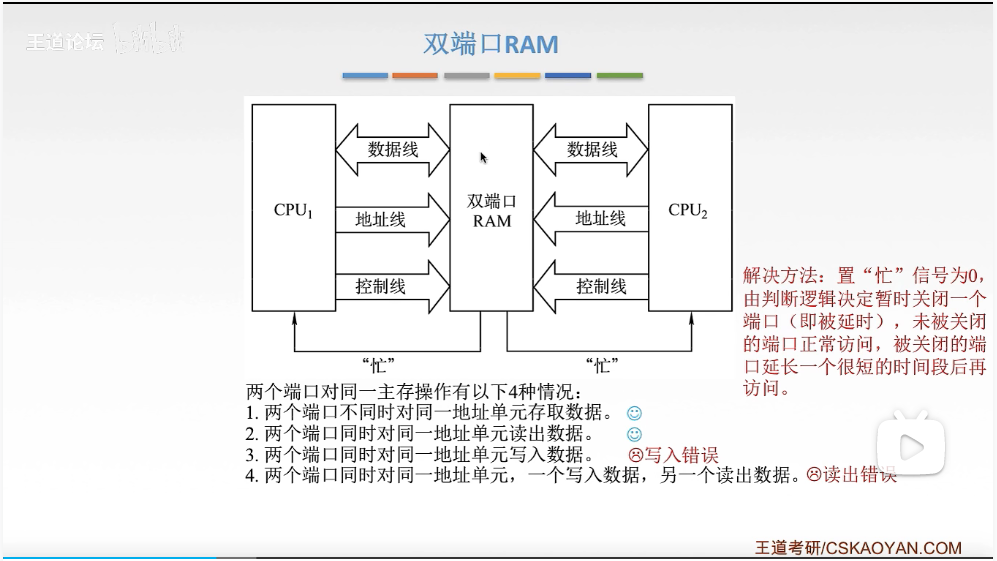
\includegraphics[scale=0.6]{双端口RAM.png}
    \caption{双端口RAM}
    \end{figure}
\begin{figure}[htbp]
    \centering
    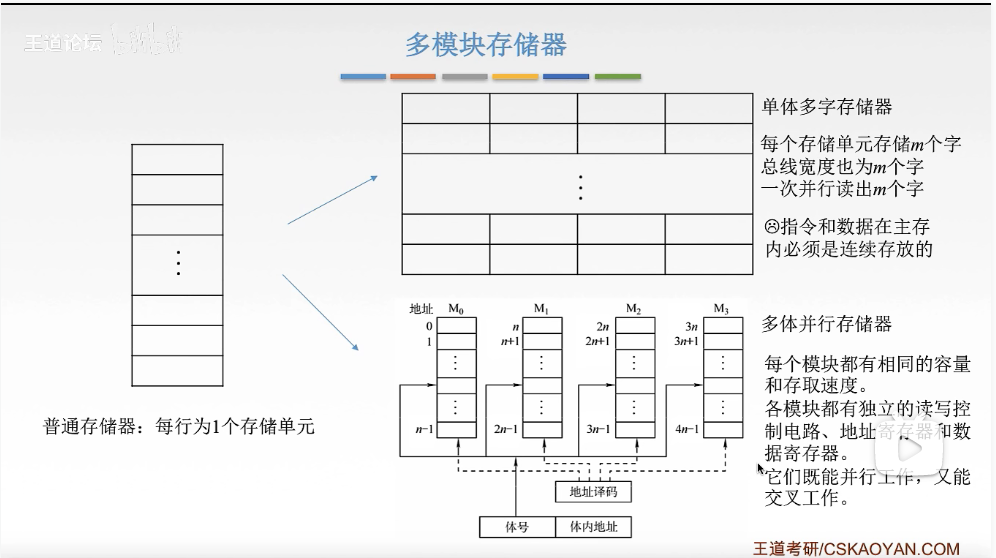
\includegraphics[scale=0.6]{多模块存储器.png}
    \caption{双端口存储器}
    \end{figure}
\begin{figure}[htbp]
    \centering
    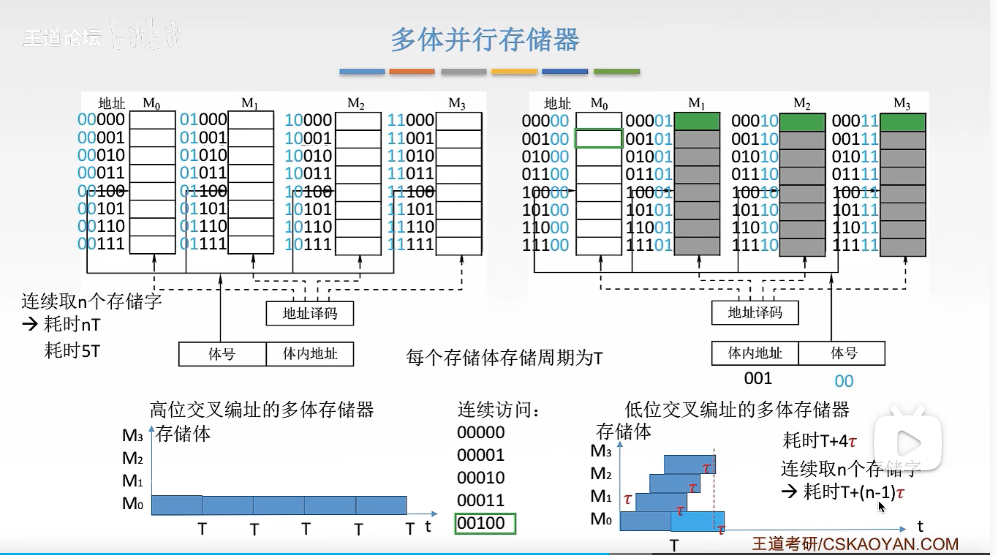
\includegraphics[scale=0.6]{多体并行存储器.png}
    \caption{多体并行存储器}
    \end{figure}
\textbf{宏观概念}为在一个存储周期内,交叉存储器可以提供的数据量为
单个模块的m倍。
\subsection{高速缓冲存储器-局部性原理性能分析}
程序访问的局部性原理 -- Cache--主存层次。

命中率H:CPU欲访问的信息已在Cache中的比率。

\begin{figure}[htbp]
    \centering
    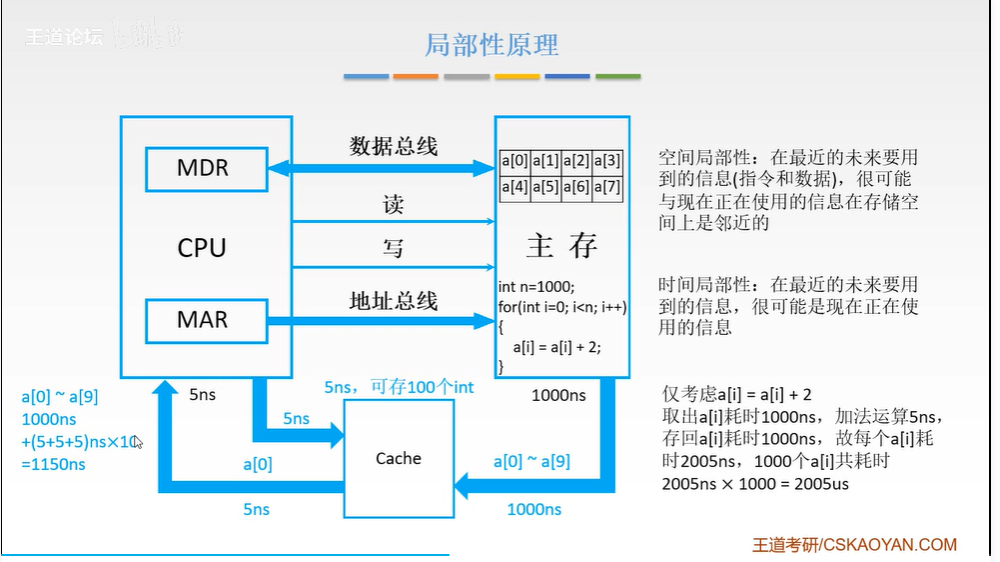
\includegraphics[scale=0.6]{局部性原理.png}
    \caption{局部性原理}
    \end{figure}
\subsection{Cache的基本工作原理}

\end{document}



